\documentclass[12pt]{article}

\usepackage{hcmus-report-template}
\usepackage{titlesec}

\setcounter{secnumdepth}{4}

\titleformat{\paragraph}
{\normalfont\normalsize\bfseries}{\theparagraph}{1em}{}
\titlespacing*{\paragraph}
{0pt}{3.25ex plus 1ex minus .2ex}{1.5ex plus .2ex}
% \usepackage{IEEEtran}
% \documentclass[conference]{IEEEtran}

% Disable indentation on new paragraphs
\setlength{\parindent}{0pt}

% Line spacing 1.5
\renewcommand{\baselinestretch}{1.5}

% Optional: graphic path
% \graphicspath{PATH_TO_GRAPHIC_FOLDER}

% To use Times font family, uncomment this row
% \usepackage{mathptmx}

% To use roman section / subsection, uncomment these rows
% \renewcommand{\thesection}{\Roman{section}}
% \renewcommand{\thesubsection}{\thesection.\Roman{subsection}}

% Define course name, report name and report title.
\newcommand{\coursename}{Hệ thống máy tính}
\newcommand{\reportname}{Reverse Engineering}
\newcommand{\reporttitle}{Báo cáo đồ án}

\newcommand{\studentname}{
\begin{tabular}{l l} % Two columns: left-aligned
Nguyễn Minh Hiếu & 23120124 \\
Huỳnh Mạnh Tường & 23120105 \\
Nguyễn Thanh Phong & 23120154 \\
\end{tabular}
                        }
\newcommand{\teachername}{Lê Viết Long}

% Header
\lhead{\reportname}
\rhead{
Trường Đại học Khoa học Tự nhiên - ĐHQG HCM\\
\coursename
}

% Footer
% \newcommand{\leftfooter}{\LaTeX\ by \href{https://github.com/trhgquan}{Quan, Tran Hoang}}
% \lfoot{\leftfooter}

% ============ DOCUMENT ============
\renewcommand\thesection{\Roman{section}}
\renewcommand\thesubsection{\arabic{subsection}}
\begin{document}

\pagenumbering{arabic}
\setcounter{page}{1}
% \pagenumbering{roman}
\begin{titlepage}
    \newcommand{\HRule}{\rule{\linewidth}{0.5mm}}
    \centering
    
    % University and department
    \textsc{\LARGE đại học quốc gia tphcm}\\[0.25cm]
    \textsc{\LARGE trường đại học khoa học tự nhiên}\\[0.25cm]
    \textsc{\LARGE khoa công nghệ thông tin}\\[0.25cm]
    
    % Logo
    
\includegraphics[scale=.25]{img/hcmus-logo.png}
    
    % Center the title section
    \vspace*{\fill} % Pushes everything above up to fill space
    
    {
    \huge{\bfseries{\reporttitle}}\\[0.5cm]
    \Large{\bfseries{Đề tài: \reportname}}
    }\\[0.3cm]
    
    \vspace*{\fill} % Pushes everything below down to fill space
    
    % Course and student/teacher information
    \textbf{\large Môn học: \coursename}\\[0.5cm]
    
    \begin{minipage}[t]{0.5\textwidth}
    \begin{flushleft} \large
    \emph{Sinh viên thực hiện:}\\
    \studentname
    \end{flushleft}
    \end{minipage}
    ~
    \begin{minipage}[t]{0.4\textwidth}
    \begin{flushright} \large
    \emph{Giáo viên hướng dẫn:} \\
    \teachername
    \end{flushright}
    \end{minipage}\\[1cm]
    
    % Date
    {\large \today}\\[1cm]
    
    \vfill
    \end{titlepage}
    

\tableofcontents
\pagebreak
% \listoftables
% \pagebreak
% \listoffigures
% \pagebreak

\section{Giới thiệu}

Ứng dụng điều khiển client-server từ xa thông qua Gmail và giao thức socket là một giải pháp kết hợp giữa công nghệ email và giao tiếp mạng nhằm thực hiện các lệnh điều khiển từ xa một cách đơn giản và hiệu quả. Quy trình hoạt động của hệ thống bao gồm:

\begin{itemize}
    \item \textbf{Admin} gửi lệnh điều khiển thông qua Gmail đến tài khoản email của \textbf{client}.
    \item \textbf{Client} tự động đọc email, phân tích nội dung lệnh, sau đó sử dụng socket để truyền lệnh này tới \textbf{server}.
    \item \textbf{Server} tiếp nhận lệnh, thực thi, xử lý kết quả, và gửi phản hồi lại cho \textbf{client}.
    \item \textbf{Client} tiếp tục gửi kết quả phản hồi thông qua email tới tài khoản Gmail của \textbf{admin}.
\end{itemize}

Hệ thống sử dụng Gmail API để thực hiện các thao tác quản lý email như nhận email, xử lý nội dung và gửi email phản hồi. Bên cạnh đó, giao thức socket được sử dụng để thiết lập kết nối trực tiếp giữa \textbf{client} và \textbf{server}, đảm bảo việc truyền tải dữ liệu diễn ra nhanh chóng và chính xác.

Ứng dụng được xây dựng hoàn toàn bằng ngôn ngữ lập trình \textbf{C/C++}, một ngôn ngữ mạnh mẽ với khả năng xử lý dữ liệu hiệu quả, hỗ trợ lập trình đa luồng và tương tác với các giao thức mạng. Với thiết kế linh hoạt, hệ thống phù hợp để triển khai trong các môi trường yêu cầu điều khiển từ xa, đồng thời đảm bảo tính bảo mật nhờ sử dụng các cơ chế xác thực của Gmail.

\newpage
\section{Phân tích thuật toán và phát triển chương trình keygen}

\subsection{File 1}
\subsubsection{Mô tả thuật toán phát sinh khóa}

\subsubsection{Chương trình phát sinh khóa}
\newpage

\subsection{File 2}
\subsubsection{Mô tả thuật toán phát sinh khóa}

\noindent\textbf{2.1.1\quad Yêu cầu}
\begin{itemize}
    \item File cần crack: \texttt{WinCrackMe.exe}
    \item Công cụ sử dụng: \texttt{OllyDbg}
    \item File GENKEY cho chương trình: \texttt{crack2.exe}
\end{itemize}

\noindent\textbf{2.1.2\quad Hướng dẫn}
\begin{itemize}
    \item Khởi động chương trình bằng cách double-click vào file \texttt{WinCrackMe.exe}. Lúc này giao diện chương trình sẽ hiển thị như sau:
    \begin{figure}[H]
        \centering
        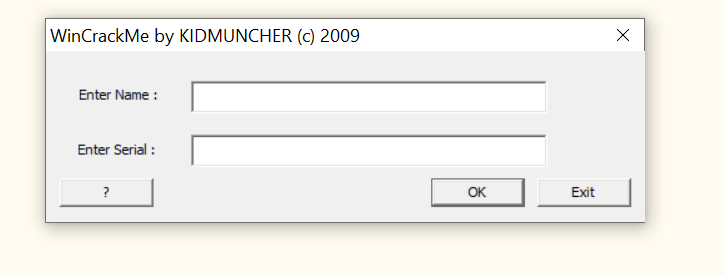
\includegraphics[width=\textwidth]{img/file-2/demo1.PNG}
        \caption{Giao diện chính của chương trình}
        \label{fig:main_interface}
    \end{figure}
    
    \item Chương trình hiển thị một hộp thoại chứa hai thuộc tính cần nhập vào (không bắt buộc): \texttt{Enter Name} và \texttt{Enter Serial}. 
    \item Bên trái dưới cùng là nút \texttt{'?'} hiển thị hướng dẫn, bên phải là nút \texttt{OK} và \texttt{Exit}.
    \begin{figure}[H]
        \centering
        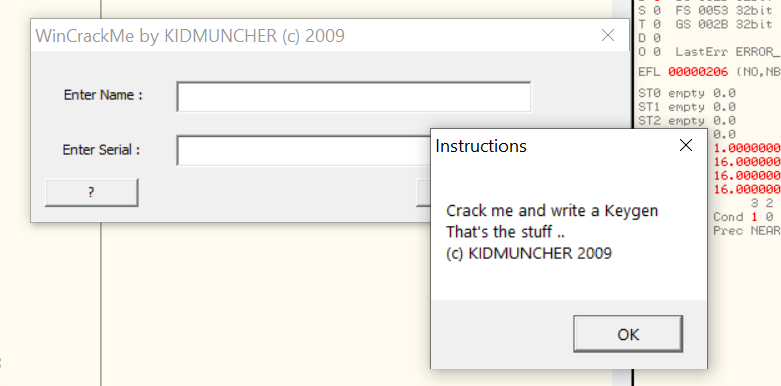
\includegraphics[width=\textwidth]{img/file-2/demo2.PNG}
        \caption{Hướng dẫn sử dụng chương trình}
    \end{figure}

    \item Các trường hợp có thể xảy ra:
    \begin{enumerate}[label=\textbf{TH\arabic*:}]
        \item Để trống cả hai thuộc tính:
        \begin{figure}[H]
            \centering
            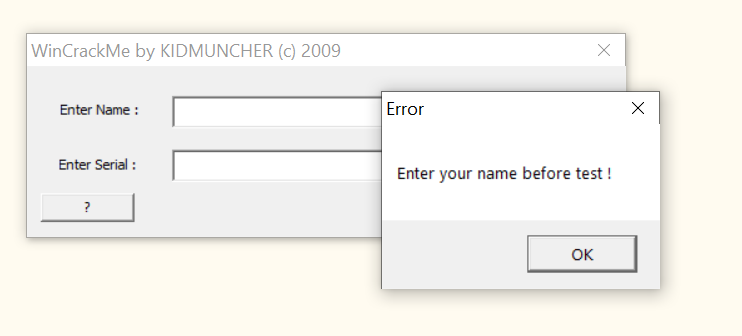
\includegraphics[width=0.8\textwidth]{img/file-2/demo3.PNG}
            \caption{Cả Name và Serial đều trống}
        \end{figure}
        
        \item Nhập \texttt{Name} với ít hơn 5 ký tự:
        \begin{figure}[H]
            \centering
            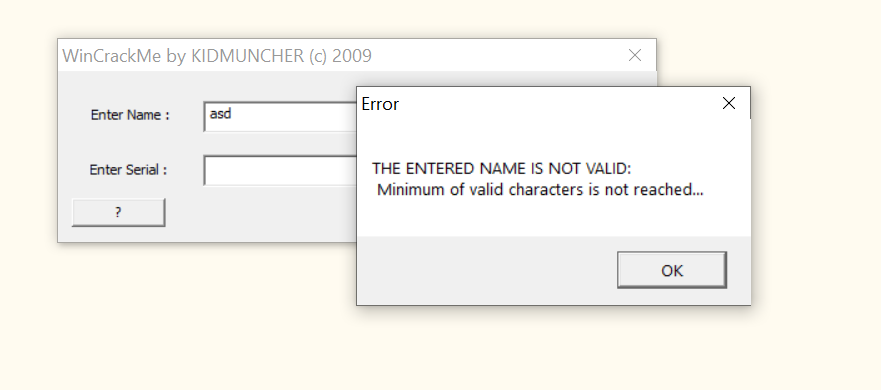
\includegraphics[width=0.8\textwidth]{img/file-2/demo4.PNG}
            \caption{Tên quá ngắn}
        \end{figure}
        
        \item Nhập \texttt{Name} chỉ gồm ký tự \texttt{a} hoặc \texttt{A}, đủ 5 ký tự:
        \begin{figure}[H]
            \centering
            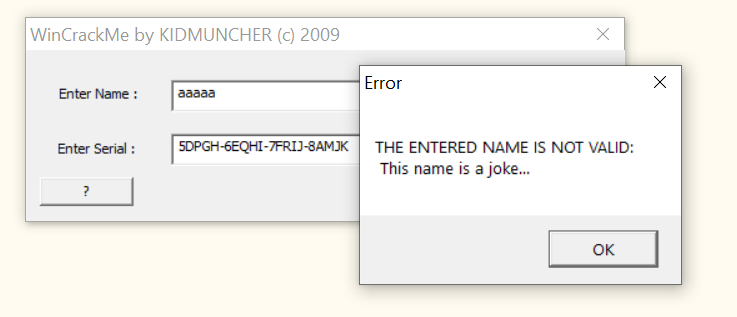
\includegraphics[width=0.8\textwidth]{img/file-2/demo5.PNG}
            \caption{Tên không đủ tốt}
        \end{figure}
        
        \item Nhập \texttt{Name} bất kỳ lớn hơn 5 ký tự:
        \begin{figure}[H]
            \centering
            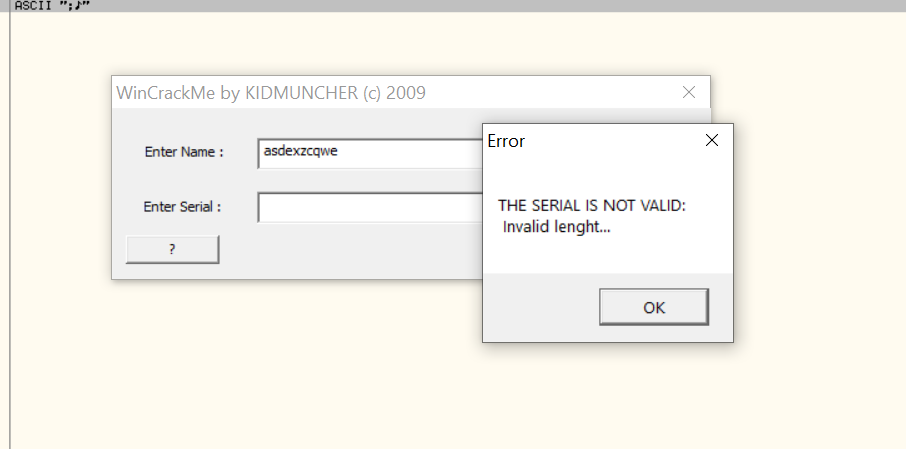
\includegraphics[width=0.8\textwidth]{img/file-2/demo6.PNG}
            \caption{Name hợp lệ nhưng Serial trống}
        \end{figure}
        
        \item Nhập \texttt{Serial} không đúng 23 ký tự:
        \begin{figure}[H]
            \centering
            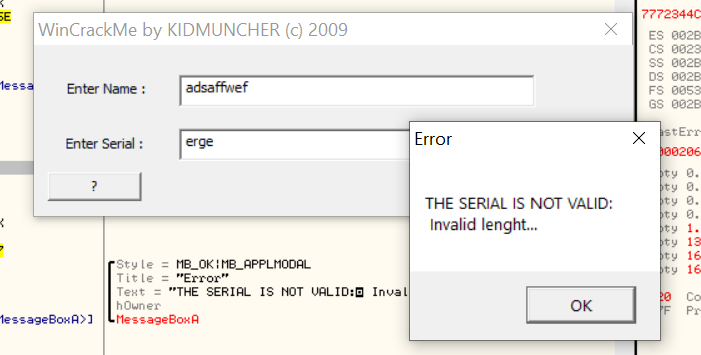
\includegraphics[width=0.8\textwidth]{img/file-2/demo9.PNG}
            \caption{Serial không đúng độ dài}
        \end{figure}
        
        \item Nhập \texttt{Serial} đúng 23 ký tự bất kỳ:
        \begin{figure}[H]
            \centering
            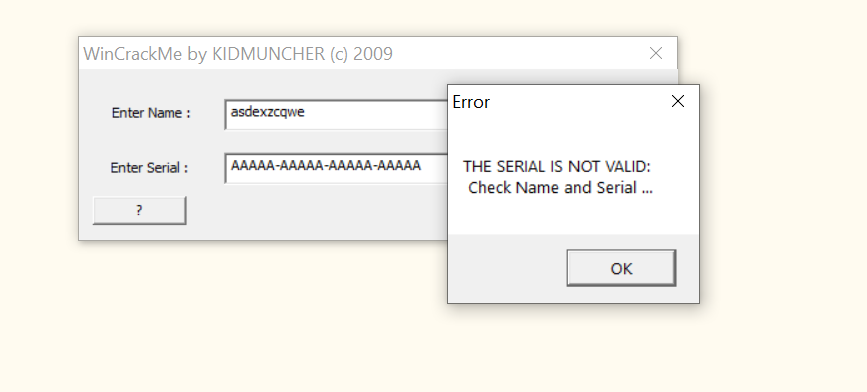
\includegraphics[width=0.8\textwidth]{img/file-2/demo7.PNG}
            \caption{Serial không hợp lệ}
        \end{figure}
        
        \item Nhập \texttt{Name} và \texttt{Serial} phù hợp:
        \begin{figure}[H]
            \centering
            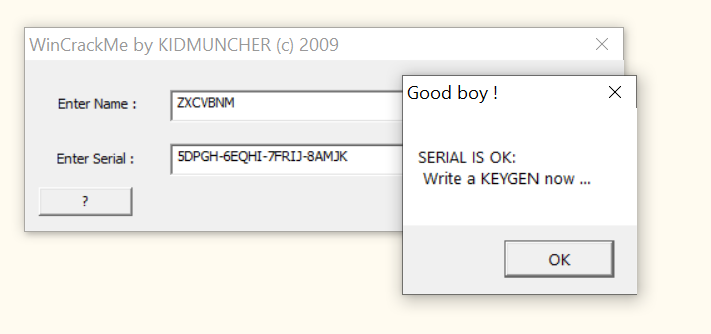
\includegraphics[width=0.8\textwidth]{img/file-2/demo8.PNG}
            \caption{Đăng nhập thành công}
        \end{figure}
    \end{enumerate}
\end{itemize}

\newpage
\noindent\textbf{2.1.3\quad Chi tiết phân tích chương trình}

\begin{itemize}
    \item Mở file \texttt{WinCrackMe.exe} bằng \texttt{OllyDbg}.
    \item Click chuột phải $\rightarrow$ \texttt{Search for > All referenced text strings}.
    \begin{figure}[H]
        \centering
        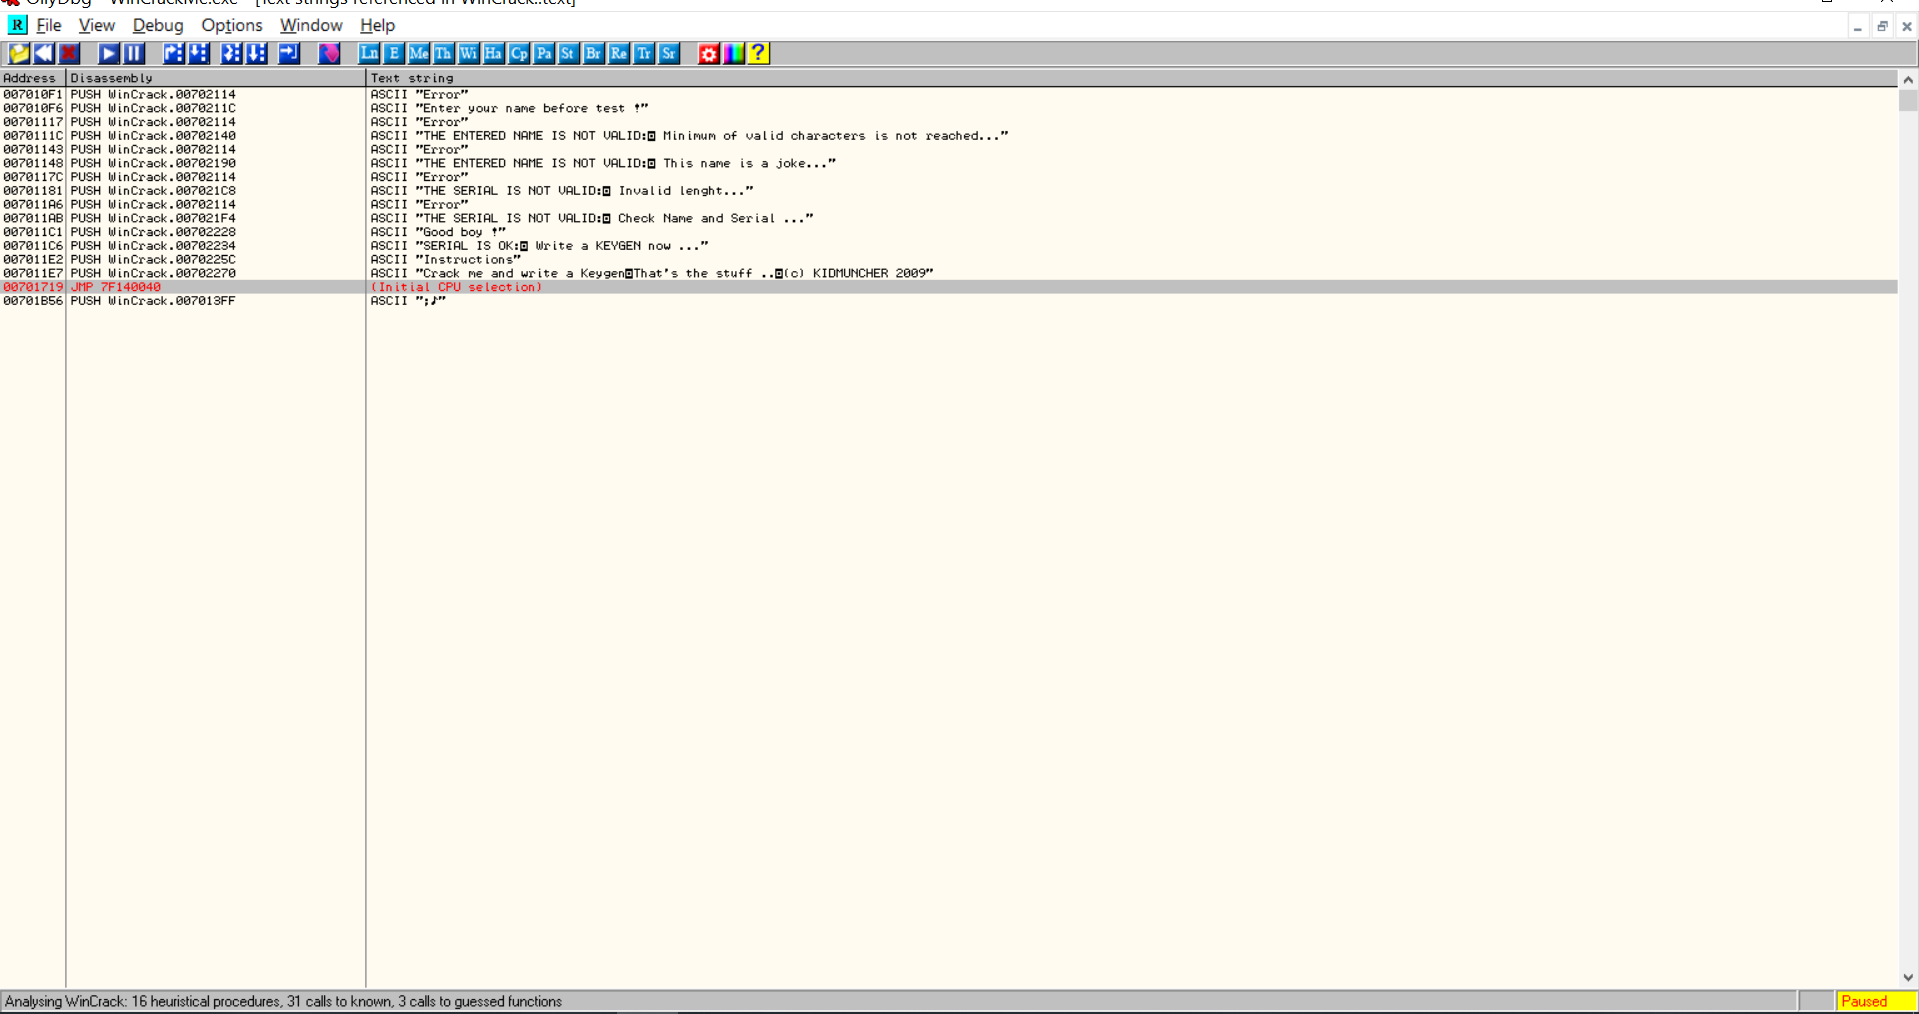
\includegraphics[width=\textwidth]{img/file-2/asm2.PNG}
        \caption{Danh sách chuỗi văn bản trong chương trình}
    \end{figure}
    
    \item Đặt Breakpoint tại đoạn code đầu tiên.
\end{itemize}

Các bước thực thi:
\begin{enumerate}[label=\textbf{Bước \arabic*:}]
    \item Nhập dữ liệu và nhấn \texttt{OK}. Chương trình dùng \texttt{GetDlgItemTextA} để lấy \texttt{Name} và \texttt{Serial}.
    \begin{center}
        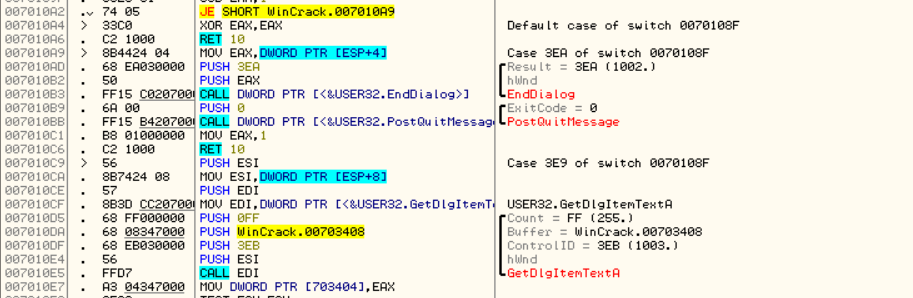
\includegraphics[width=0.8\textwidth]{img/file-2/asm3.PNG}
    \end{center}

    \item Kiểm tra \texttt{Name} có rỗng không với lệnh \texttt{TEST EAX, EAX}.
    \begin{center}
        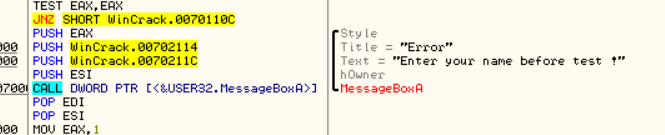
\includegraphics[width=0.8\textwidth]{img/file-2/asm4.PNG}
    \end{center}

    \item Kiểm tra số lượng ký tự chữ cái trong \texttt{Name} $\geq$ 5.
    \begin{center}
        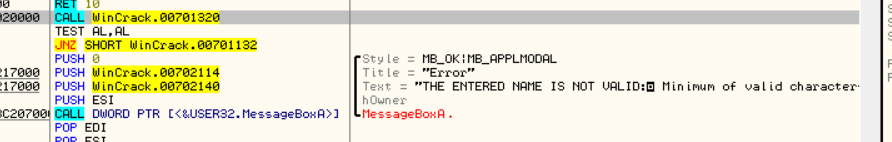
\includegraphics[width=0.8\textwidth]{img/file-2/asm5.PNG}
    \end{center}

    \item Tính giá trị \texttt{hash} từ \texttt{Name}.
    \begin{center}
        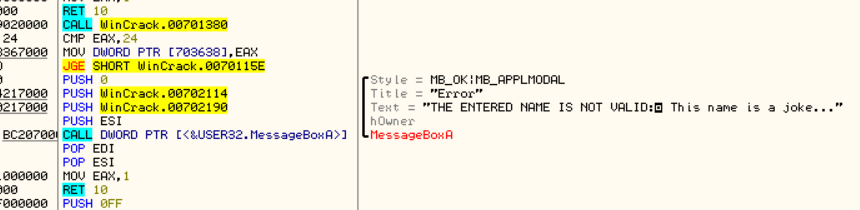
\includegraphics[width=0.8\textwidth]{img/file-2/asm6.PNG}
    \end{center}

    \item Kiểm tra độ dài \texttt{Serial} đúng bằng 23 ký tự.
    \begin{center}
        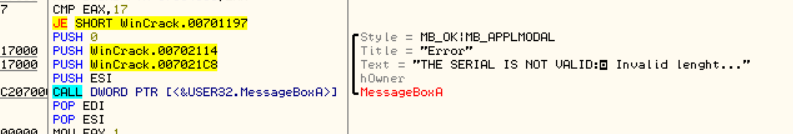
\includegraphics[width=0.8\textwidth]{img/file-2/asm7.PNG}
    \end{center}

    \item Tính \texttt{hash} từ \texttt{Serial} và so sánh với \texttt{hash} từ \texttt{Name}.
    \begin{center}
        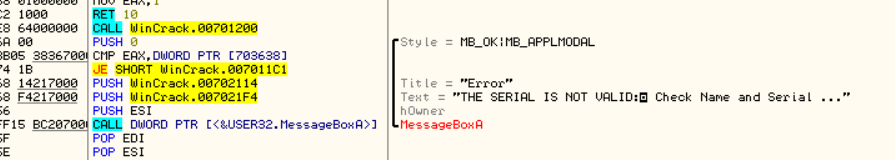
\includegraphics[width=0.8\textwidth]{img/file-2/asm8.PNG}
    \end{center}

    \item Nếu trùng khớp, hiển thị thông báo thành công.
    \begin{center}
        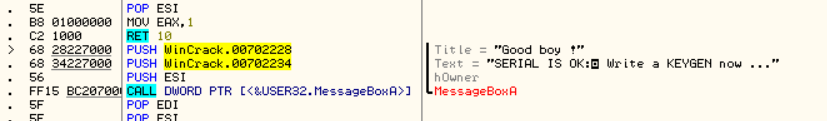
\includegraphics[width=0.8\textwidth]{img/file-2/asm9.PNG}
    \end{center}
\end{enumerate}

\subsubsection{Thuật toán phát sinh khóa}

\begin{itemize}
    \item \textbf{Tính hash của Name}:
        \begin{itemize}
        \item Hàm tính hash từ thuộc tính Name trong chương trình:
    \end{itemize}
        \begin{center}
        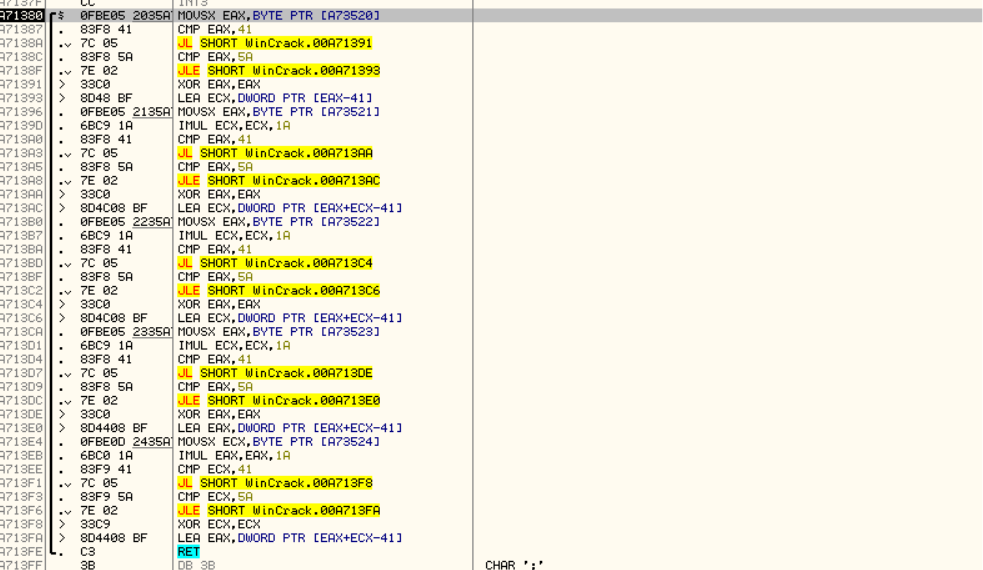
\includegraphics[width=0.8\textwidth]{img/file-2/asm11.PNG}
    \end{center}
    \begin{itemize}
        \item Chương trình sẽ kiểm tra các kí tự sao cho chúng là chữ cái in hoa hoặc in thường trong bảng ASCII. Các kí tự này đã được kiểm tra từ trước.
        \item Lấy 5 ký tự chữ cái đầu tiên, sau đó tính giá trị của nó dựa trên vị trí của chúng trong bảng chữ cái Alphabet. Lưu ý, các giá trị trong đoạn code trên dưới dạng HEX.
        \item Công thức tính giá trị hash như sau:
        \[
        hash = hash \times 1A + (\text{lower}(ch[i]) - 'a')(HEX)
        \]
        \[
        hash = hash \times 26 + (\text{lower}(ch[i]) - 'a')(DEC)
        \]
    \end{itemize}
    \begin{center}
        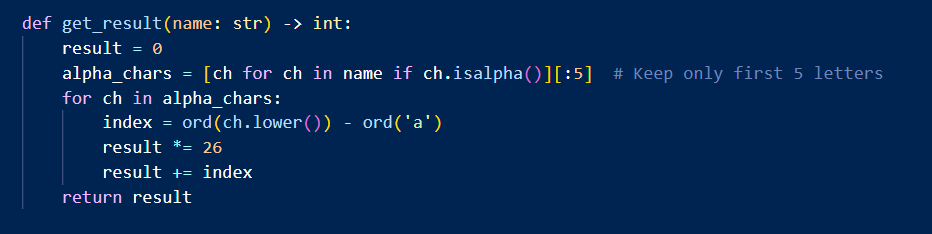
\includegraphics[width=0.8\textwidth]{img/file-2/code1.PNG}
    \end{center}
    
    \item \textbf{Tính hash của Serial}:
    \begin{itemize}
        \item Serial có 23 ký tự, chia thành 4 nhóm, mỗi nhóm 5 ký tự, ngăn cách bởi 1 dấu gạch ngang \texttt{-}.
        \item Sử dụng 4 bảng hash khác nhau ứng với từng nhóm, với mỗi bảng hash được rotate 1 đoạn cố định so với bảng hash trước.
        \item Công thức băm từng nhóm:
    \end{itemize}
    \begin{center}
        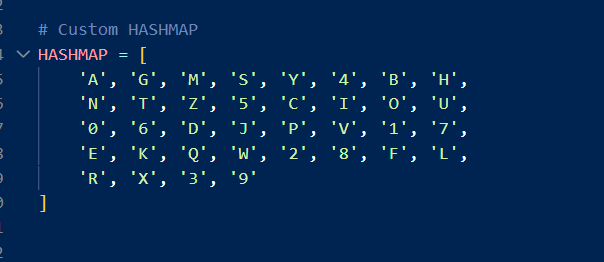
\includegraphics[width=0.8\textwidth]{img/file-2/code2.PNG}
        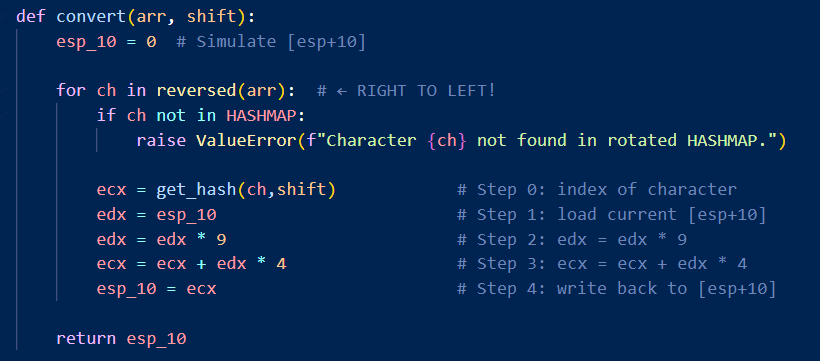
\includegraphics[width=0.8\textwidth]{img/file-2/code3.PNG}        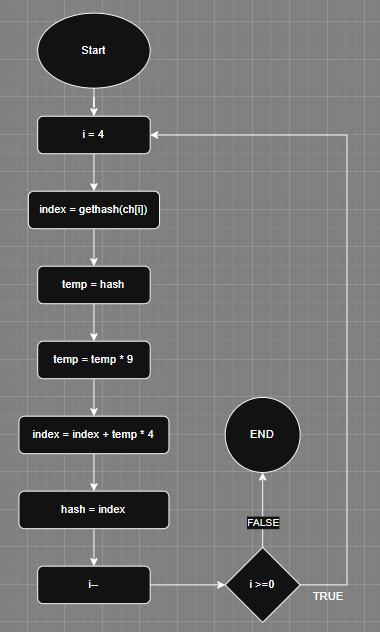
\includegraphics[width=0.8\textwidth]{img/file-2/img1.PNG}
    \end{center}

    \item \textbf{Điều kiện thành công}:
    \begin{itemize}
        \item Hash của tất cả 4 nhóm phải bằng nhau.
        \item Hash này phải trùng với hash của \texttt{Name}.
    \end{itemize}

    \item \textbf{Chương trình GENKEY}:
    \begin{itemize}
        \item Sử dụng thuật toán tham lam (\textit{Greedy Algorithm}) để tìm 1 giá trị Serial phù hợp với Name.
        \item Nhập Name vào chương trình GENKEY, Số Serial phù hợp được lưu vào file \texttt{key.txt}. 
    \end{itemize}
\end{itemize}

\newpage
\subsubsection{Kết luận}

Chương trình \texttt{WinCrackMe.exe} sử dụng kỹ thuật \textbf{hashing} để mã hóa và kiểm tra tính hợp lệ của dữ liệu đầu vào. Cụ thể:

\begin{itemize}
    \item Dữ liệu \texttt{Name} được xử lý bằng một hàm hash tuyến tính đơn giản, dựa trên 5 ký tự đầu tiên.
    \item Dữ liệu \texttt{Serial} được chia thành các nhóm, mỗi nhóm sử dụng một hàm băm phức tạp hơn với nhiều phép toán nhân, cộng và bảng ánh xạ riêng biệt, nhằm tạo ra tính ngẫu nhiên và tăng độ khó cho việc dò tìm bằng phương pháp brute-force.
    \item Cơ chế kiểm tra thành công dựa trên việc so khớp toàn bộ các giá trị hash đã tính từ \texttt{Name} và từng nhóm của \texttt{Serial}.
\end{itemize}

Việc phân tích mã assembly bằng công cụ \texttt{OllyDbg} giúp làm rõ luồng thực thi của chương trình và cách các hàm API Windows như \texttt{GetDlgItemTextA} được sử dụng để thu thập dữ liệu từ giao diện người dùng.

Bằng cách hiểu rõ thuật toán hashing nội tại, chúng tôi đã thiết kế được một chương trình \textbf{GENKEY} hoạt động hiệu quả, cho phép tự động sinh ra các cặp \texttt{Name} - \texttt{Serial} hợp lệ, đáp ứng mọi yêu cầu xác thực của ứng dụng.

\bigskip
\noindent\textbf{Ý nghĩa thực tiễn}:
\begin{itemize}
    \item Củng cố kỹ năng phân tích mã máy và dịch ngược (reverse engineering).
    \item Nâng cao kiến thức về kỹ thuật bảo mật phần mềm thông qua các thuật toán mã hóa nhẹ (lightweight hashing).
    \item Minh họa cách xây dựng công cụ hỗ trợ (GENKEY) dựa trên việc khai thác logic nội bộ của chương trình mục tiêu.
\end{itemize}

\bigskip
\noindent\textbf{Đánh giá tổng quát}: \\
Chương trình có mức độ bảo vệ cơ bản, chủ yếu dựa vào sự phức tạp của hàm băm hơn là cơ chế mã hóa mạnh mẽ. Với kiến thức về dịch ngược và phân tích thuật toán, việc xây dựng keygen phù hợp hoàn toàn khả thi.


\newpage

\subsection{File 3}
\subsubsection{Mô tả thuật toán phát sinh khóa}

\subsubsection{Chương trình phát sinh khóa}
\newpage
\section{Đánh giá mức độ hoàn thành}

\begin{table}[H]
    \centering
    \begin{tabular}{|c|c|c|c|}
    \hline
    \textbf{Tên bài} & \textbf{Mức độ hoàn thành (\%)} & \textbf{Người phụ trách} & \textbf{Mã số sinh viên} \\ \hline
    file-1 & 100\% & Nguyễn Thanh Phong & 23120154 \\ \hline
    file-2 & 100\% & Huỳnh Mạnh Tường & 23120105 \\ \hline
    file-3 & 100\% & Nguyễn Minh Hiếu & 23120124 \\ \hline
    \end{tabular}
    \caption{Bảng đánh giá mức độ hoàn thành}
    \label{tab:hoanthanh}
\end{table}

% References
% \cleardoublepage
\phantomsection
\addcontentsline{toc}{section}{Tài liệu}
\bibliographystyle{plain}
\bibliography{ref/ref}


% Appendix
% \appendix
% Add \cleardoublepage to move appendices to next page.
%\section{Phụ lục}
\begin{itemize}
\item Template này \textbf{không phải} là template chính thức của Khoa Công nghệ thông tin - Trường Đại học Khoa học Tự nhiên.
\item Các hình ảnh, bảng biểu, thuật toán trong template chỉ mang tính chất ví dụ.
\item Nhóm tác giả phân phối \textbf{miễn phí} template này \href{https://github.com/khongsomeo/hcmus-unofficial-report-template}{trên GitHub} và \href{https://www.overleaf.com/latex/templates/hcmus-report-template/zyrhmsxynwqs}{trên Overleaf} với \href{https://github.com/khongsomeo/hcmus-unofficial-report-template/blob/main/LICENSE}{Giấy phép GNU General Public License v3.0}. Nhóm tác giả không chịu trách nhiệm với các bản phân phối không nằm trong hai kênh phân phối chính thức nêu trên.
\end{itemize}

\end{document}